\documentclass{beamer}
\usetheme{Dresden}
\usefonttheme[onlymath]{serif}

%\input{examplepages.tex}

\usepackage{graphicx}
\usepackage{xcolor}
\usepackage{adjustbox}
\usepackage{fontawesome5}
\usepackage{tikz}
	\usetikzlibrary{patterns}
\usepackage{shapepar}
%\usepackage{hologo}
%\usepackage{showexpl}
\usepackage{hyperref}
\usepackage{tcolorbox}
\usepackage{enumitem}
	\setitemize{label=\usebeamerfont*{itemize item}%
	\usebeamercolor[fg]{itemize item}
	\usebeamertemplate{itemize item}}
%\usepackage{calc}
\usepackage{nth}
\usepackage{siunitx}
%\usepackage{fp}
\usepackage{mhchem}
\usepackage{chemfig}
\usepackage{bibentry}
\usepackage{soul}







%%%%%%%%%%%%%% TITLE BLOCK
\title{On Sustainability as a Cyber-Physical-Social System}
\subtitle{The XGEM Initiative Multiscale Integration of Methane Monitoring for Impact Characterization and Mitigation}
%\thanks{\href{https://github.com/BlueNalgene/Introduction_to_LaTeX}{https://github.com/BlueNalgene/Introduction\_to\_LaTeX}}
\author{Wesley T. Honeycutt}
\institute{Systems Realization Laboratory Conversations Series\\University of Oklahoma}
\date{September \nth{19}, 2021}







%%%%%%%%%%%%%% COLOR DEFINITIONS
\definecolor{OUCrimson}{RGB}{132 22 23} % UBC Blue (primary)
\definecolor{OUCream}{RGB}{253 249 216} % UBC Grey (secondary)







%%%%%%%%%%%%%% BEAMER FORMATTING
\setbeamercolor{palette primary}{bg=OUCrimson,fg=white}
\setbeamercolor{palette secondary}{bg=OUCrimson,fg=white}
\setbeamercolor{palette tertiary}{bg=OUCrimson,fg=white}
\setbeamercolor{palette quaternary}{bg=OUCrimson,fg=white}
\setbeamercolor{structure}{fg=OUCrimson} % itemize, enumerate, etc
\setbeamercolor{section in toc}{fg=OUCrimson} % TOC sections
\setbeamerfont{footnote}{size=\tiny}
\setbeamertemplate{bibliography entry article}{}
\setbeamertemplate{bibliography entry title}{}
\setbeamertemplate{bibliography entry location}{}
\setbeamertemplate{bibliography entry note}{}

% Override palette coloring with secondary
\setbeamercolor{subsection in head/foot}{bg=OUCream,fg=white}

\makeatletter
\Hy@AtBeginDocument{%
	\def\@pdfborder{0 0 1}% Overrides border definition set with colorlinks=true
	\def\@pdfborderstyle{0 0 0}% Overrides border style set with colorlinks=true
	% Hyperlink border style will be underline of width 1pt
}
\makeatother

\hypersetup{%
	colorlinks=true,% hyperlinks will have color
	linkcolor=blue,
	urlcolor=blue,
	linkbordercolor=blue,% hyperlink borders will be red
	pdfborderstyle={/S/U/W 0}% border style will be underline of width 1pt
}







%%%%%%%%%%%%%% TIKZ FUNCTIONS
\usetikzlibrary{calc,fit,intersections}
\newcommand{\metalone}{[pattern= horizontal lines, pattern color=blue]}
\newcommand{\metaltwo}{[pattern= vertical lines, pattern color=purple]}
\newcommand{\poly}{[pattern= grid, pattern color=red]}
\newcommand{\pdiff}{[pattern= north east lines, pattern color=orange]}
\newcommand{\ndiff}{[pattern= north west lines, pattern color=green]}
\newcommand{\pwell}{[pattern= crosshatch dots, pattern color=orange]}
\newcommand{\nwell}{[pattern= crosshatch dots, pattern color=green]}
\newcommand{\oxide}{[pattern = bricks, pattern color = olive]}
\newcommand{\silicon}{[fill = white]}
\newcommand{\metalthree}{[fill = teal]}
\def\shapeparnodeaccuracy{2}
\newcommand\shapeparnode[6][]{
	% 6 parameters:
	% style for node (default:empty),
	% h margin, v margin, left path, right path, text (just one paragraph!)
	
	% name left and right paths and compute there bounding boxes
	\begin{scope}[local bounding box=leftbb]
		\path[name path global=left,xshift=#2] #4;
	\end{scope}
	\node[inner ysep=-#3,inner xsep=0pt,fit=(leftbb)](leftbb){};
	\begin{scope}[local bounding box=rightbb]
		\path[name path global=right,xshift=-#2] #5;
	\end{scope}
	\node[inner ysep=-#3,inner xsep=0pt,fit=(rightbb)](rightbb){};
	
	% global bounding box
	\path let
	\p1=(leftbb.north west), \p2=(leftbb.south west),
	\p3=(rightbb.north east), \p4=(rightbb.south east)
	in
	\pgfextra{
		\pgfmathsetmacro{\ymin}{(\y1 < \y3) ? \y1 : \y3}
		\pgfmathsetmacro{\ymax}{(\y2 > \y4) ? \y2 : \y4}
		\typeout{ymin \ymin}
		\typeout{ymax \ymax}
	} node[inner sep=0,fit={(\x1,\ymin pt)(\x3,\ymax pt)}](mybb){};
	
	% compute nb steps
	\path let \p1=(mybb.north), \p2=(mybb.south) in
	\pgfextra{
		\pgfmathsetmacro{\fnthght}{1em/\shapeparnodeaccuracy}
		\pgfmathtruncatemacro{\nbsteps}{(\y1-\y2)/\fnthght}
		\xdef\nbsteps{\nbsteps}
		\typeout{nb steps \nbsteps}
	};
	
	% horizontal references
	\path (mybb.north) -- (mybb.south)
	\foreach \cnt in {0,1,...,\nbsteps}{
		\pgfextra{\pgfmathsetmacro{\pos}{\cnt/\nbsteps}}
		coordinate[pos=\pos] (ref \cnt)
	};
	
	% left and right boundaries coordinates
	\foreach \cnt in {0,1,...,\nbsteps}{
		% an horizontal line from left to right
		\path[name path=ltor]
		(mybb.west |- ref \cnt) --  (mybb.east |- ref \cnt);
		% same line from right to left
		\path[name path=rtol]
		(mybb.east |- ref \cnt) -- (mybb.west |- ref \cnt);
		% left boundary
		\path[name intersections={of=rtol and left,by={l \cnt},sort by=rtol}];
		% right boundary
		\path[name intersections={of=ltor and right,by={r \cnt},sort by=ltor}];
	}
	% start point (and initial value of boundshape)
	\path let \p1=(l 0) in 
	\pgfextra{
		\pgfmathsetmacro{\xstart}{\x1}
		\xdef\boundshape{{0}{0}b{\xstart}}
		\xdef\xmin{\xstart}
		\xdef\xmax{\xstart}
	};
	
	% top and bottom
	\path let \p1=(l 0), \p2=(l \nbsteps) in
	\pgfextra{
		\pgfmathsetmacro{\ystart}{\y1}\xdef\ystart{\ystart}
		\pgfmathsetmacro{\yending}{\y2}\xdef\yending{\yending}
	};
	% incremental definition of boundshape
	\foreach \cnt in {0,1,...,\nbsteps}{
		\path let \p1=(l \cnt), \p2=(r \cnt) in
		\pgfextra{
			\pgfmathsetmacro{\start}{\x1}
			\pgfmathsetmacro{\len}{\x2-\x1}
			\pgfmathsetmacro{\ypos}{\cnt/\nbsteps*(\ystart - \yending)}
			{\let\\=\relax \xdef\boundshape{\boundshape\\{\ypos}t{\start}{\len}}}
			\pgfmathsetmacro{\xmin}{(\xmin < \start) ? \xmin : \start}
			\xdef\xmin{\xmin}
			\pgfmathsetmacro{\xmax}{(\xmax > \start + \len) ? \xmax : \start + \len}
			\xdef\xmax{\xmax}
		};
	}
	% draw the node with text in a shapepar
	\pgfmathsetmacro{\ymax}{\ystart - \yending}
	{\let\\=\relax \xdef\boundshape{\boundshape\\{\ymax}e{0}}}
	\node[#1,text width=\xmax pt - \xmin pt,align=flush left,
	anchor=north west,inner sep=0]
	at (mybb.north west -| \xmin pt,0)
	{\Shapepar[1pt]{\boundshape}#6\par};
}
\newcommand\sbullet[1][.5]{\mathbin{\vcenter{\hbox{\scalebox{#1}{$\bullet$}}}}}






%%%%%%%%%%%%%% IMAGE PATH
\graphicspath{ {images/} } %this removes clutter from the root folder








\begin{document}
	
	\frame{\titlepage
%			\footnotetext{\href{https://github.com/BlueNalgene/Introduction_to_LaTeX}{https://github.com/BlueNalgene/Introduction\_to\_LaTeX}}
		}
	
	\frame{\tableofcontents}
	
	\section{Why Methane?}
	
		\frame{\frametitle{Methane (\ce{CH4}) Basics}
			\begin{columns}
				\column{\linewidth/3*2}
					\begin{itemize}
						\item Simplest aliphatic compound
						\item Colorless, odorless
						\item $T_{bp}$=\SI{161.5}{\degreeCelsius}
						\item Fuel source \\ \ce{CH4 + 2O2 ->[$\Delta$] CO2 + 2H2O}; $\Delta{}H=$\SI{-891}{\kilo\joule\per\mole}
						\item Feedstock for many chemical processes
					\end{itemize}
				\column{\linewidth/3}
					\begin{center}
						\chemfig{C(-[1]H)(-[3]H)(<[5]H)(<:[7]H)}
					\end{center}
			\end{columns}
		}
	
		\frame{\frametitle{Emissions}
			\begin{itemize}
				\item Naturally by abiotic geochemical processes
				\item Biotic output
				\begin{itemize}
					\item Methanogens (bacteria, archaea)
					\item Ruminants
					\item Minor sources: termites, rice, many other vertebrates
				\end{itemize}
				\item By-product of chemical syntheses
				\item Leakage
			\end{itemize}
			\begin{tcolorbox}[colback=OUCrimson!5,colframe=OUCrimson,title=Greenhouse Gas]
				\ce{CH4} is responsible for about 20\% of radiative forcing.
			\end{tcolorbox}
		}

		\frame{\frametitle{The Web of Climate Action Failure}
			\begin{center}
				\includegraphics[
				width=\linewidth,
				height=\linewidth/2,
				keepaspectratio]{risk_interconnection.jpg}
			\end{center}
			\let\thefootnote\relax\footnotetext{World Economic Forum Global Risks Interconnection Map, 2020}
		}
	
	
	
	\section{Many Atmospheric Scales}
		
		\frame{\frametitle{Top-Down and Bottom-Up}
			\begin{tikzpicture}
			\def\arroneleft{(4.5,3) to (4.5,-1) to (4,-1) to (6,-3)}
			\def\arroneright{(8,-1) to (7.5,-1) to (7.5,3)}
			\def\arrtwoleft{(12,3) to (10,1) to (10.5,1) to (10.5,-3)}
			\def\arrtworight{(13.5,-3) to (13.5,1) to (14,1)}
			\only<1->{\shapeparnode{1em}{.2em}{\arroneleft}{\arroneright}{%
			$\bullet$Atmospheric\\measurement\\
			$\bullet$~Transport\\models\\
			$\bullet$~Climate\\Reports}}
			\only<1->\draw[blue, ultra thick] \arroneleft -- \arroneright -- cycle;
			\only<2>{\shapeparnode{1em}{.2em}{\arrtwoleft}{\arrtworight}{%
			$\bullet$~Output\\inventories\\
			$\bullet$~Point\\measurements\\
			$\bullet$~Flux models}}
			\only<2>\draw[red, ultra thick] \arrtwoleft -- \arrtworight -- cycle;
			\end{tikzpicture}
		}
	
		
		\frame{\frametitle{Spatio-temporal Scales}
			\begin{center}
				\includegraphics[
				width=\linewidth,
				height=\linewidth/2,
				keepaspectratio]{spatemp.png}
			\end{center}
			\let\thefootnote\relax\footnotetext{\bibentry{nationalacademiesofsciencesImprovingCharacterizationAnthropogenic2018}}
			}
		
		\frame{\frametitle{Top-Down: Global Levels}
			\begin{center}
				\includegraphics[
				width=\linewidth/5,
				keepaspectratio]{ch4_level.png}
				\\~\\
				\includegraphics[
				width=\linewidth,
				height=\linewidth/2,
				keepaspectratio]{ch4_trend_all_gl.pdf}
			\end{center}
			}
		
		\frame{\frametitle{Top-Down: Atmospheric Predictive Models}
			\begin{tikzpicture}[remember picture,overlay]
			\node[at=(current page.center)] {
				\includegraphics[
				width=\paperwidth,
				height=\linewidth/2,
				keepaspectratio]{ch4_models.png}
			};
			\end{tikzpicture}
			\let\thefootnote\relax\footnotetext{Courtesy of Xiao-Ming Hu at OU CAPS}
			}
		
		
		\frame{
			\begin{center}
				{\Huge Does this match reality?}
			\end{center}
			}
		
		\frame{\frametitle{How do we measure this?}
			\begin{center}
				\includegraphics[
				width=\linewidth,
				height=\linewidth/2,
				keepaspectratio]{sites_2016.png}<1>
				\includegraphics[
				width=\linewidth,
				height=\linewidth/2,
				keepaspectratio]{column_measurement.png}<2>
			\end{center}
			\let\thefootnote\relax\footnotetext{\bibentry{nationalacademiesofsciencesImprovingCharacterizationAnthropogenic2018}}<1>
			\let\thefootnote\relax\footnotetext{Graphic borrowed from Wikipedia}<2>
			}
		

		\frame{\frametitle{Covering Ground}
			\begin{tikzpicture}[remember picture,overlay]
			\only<1>{
				\node[at=(current page.center)]{
					\includegraphics[
					width=\linewidth,
					height=\linewidth/2,
					keepaspectratio]{testdeploy.jpg}
				}
			};
			\only<2->{
				\node[at=(current page.center)]{
					\includegraphics[
					width=\linewidth,
					height=\linewidth/2,
					keepaspectratio]{1daych4.pdf}
				}
			};
			\only<3->{
				\node[at=(current page.east), xshift=-1.5cm]{
					\includegraphics[
					angle=-45,
					width=\linewidth/4,
					height=\linewidth/4,
					keepaspectratio]{ch4_level.png}
				}
			};
			\end{tikzpicture}
		}

		\frame{\frametitle{The Column Problem}
			\begin{tikzpicture}[remember picture,overlay]
			\node[at=(current page.center)]{
				\includegraphics[
				width=\linewidth,
				height=\linewidth/2,
				keepaspectratio]{co2_col.png}
			};
			\node[at=(current page.45), yshift=-1.5cm] {
				\includegraphics[
				width=\linewidth/4,
				height=\linewidth/4,
				keepaspectratio]{uav.png}
			};
			\end{tikzpicture}
			\let\thefootnote\relax\footnotetext{Courtesy of Elizabeth Pillar-Little at OU CIMMS}
			}
		\frame{\frametitle{Total Column Measurements Average Constituents}
			\begin{center}
				\includegraphics[
				width=\linewidth,
				height=\linewidth/2,
				keepaspectratio]{column_measurement.png}
			\end{center}
			\let\thefootnote\relax\footnotetext{Graphic borrowed from Wikipedia}
			}

		\frame{
			\begin{center}
				\only<1>{\Huge Let's just measure more columns!}
				\only<2>{\Huge \st{Let's just measure more columns!}\\ \ce{CH4} Sensor Technology is Terrible}
			\end{center}
			}
		
		\frame{\frametitle{The Duality of \ce{CH4} Sensors}
			\begin{tikzpicture}[remember picture,overlay]
			\node[at=(current page.west), xshift=2.5cm, yshift=0.5cm]{
				\includegraphics[
				width=\linewidth,
				height=\linewidth/3,
				keepaspectratio]{ch4sensorpic.png}
			};
		
			\node[at=(current page.west), xshift=2.5cm, yshift=-2.5cm, align=center]{
				$C_{LOD}=16.7$ppm\\ \$5
			};
		
			
			\node[at=(current page.east), xshift=-2.5cm, yshift=0.5cm]{
				\includegraphics[
				width=\linewidth,
				height=\linewidth/3,
				keepaspectratio]{zre.jpg}
			};
		
			\node[at=(current page.east), xshift=-2.5cm, yshift=-2.5cm, align=center]{
				$C_{LOD}=1$ppm\\ \$50,000
			};
			\end{tikzpicture}
			}
		

		\frame{
			\only<1>{\frametitle{The Blind Men and the Elephant}}
			\only<2->{\frametitle{The \st{Blind Men} Honeycutt House and the \st{Elephant} Cat}}
			\begin{picture}(320,240)
				\put(10,145){\includegraphics[
					angle=45,
					width=\linewidth/3,
					height=\linewidth/3,
					keepaspectratio
					]{gram_wes.png}<3->
				}
				\put(200,145){\includegraphics[
					width=\linewidth/3,
					height=\linewidth/3,
					keepaspectratio]{gram_claire.png}<4->
				}
				\put(10,50){\includegraphics[
					width=\linewidth/3,
					height=\linewidth/3,
					keepaspectratio
					]{gram_guest.png}<5->
				}
				\put(200,50){\includegraphics[
					width=\linewidth/3,
					height=\linewidth/3,
					keepaspectratio
					]{gram_mouse.png}<6->
				}
				\put(90,100){\includegraphics[
					width=\linewidth/3,
					height=\linewidth/3,
					keepaspectratio
					]{gram_briar.png}<7->
				}
			\end{picture}
		}
	
		\frame{\frametitle{We Need an Integrated "Whole Cat" Approach}
			\begin{center}
				\includegraphics[
				width=\linewidth,
				height=\linewidth/2,
				keepaspectratio]{xgem_integration.png}
			\end{center}
		}
	
	
	\section{Human Interaction}
		
		\frame{\frametitle{The Gift: Oklahoma Recovers from the Dustbowl}
			\begin{center}
				\includegraphics[
				width=\linewidth,
				height=\linewidth/2,
				keepaspectratio]{seminole.jpg}
			\end{center}
			\let\thefootnote\relax\footnotetext{Michael Vance1: https://www.flickr.com/photos/miklvance/46249282192/in/photostream/}
		}
		
		\frame{\frametitle{The Gift: Shale Gas Revolution}
			\begin{center}
				\includegraphics[
				width=\linewidth,
				height=\linewidth/2,
				keepaspectratio]{gas_plant.jpg}
			\end{center}
			\let\thefootnote\relax\footnotetext{\bibentry{wilmothONEOKIncBuild2018}}
		}

		\frame{\frametitle{Health Impacts of \ce{CH4}}
			
			\begin{itemize}
				\item Methane is biologically inert
				\begin{itemize}
					\item 24-h and 90-d limit is 5,000 ppm (with no explanation)
					\item Miners must evacuate at 2,500 ppm
				\end{itemize}
				\item Yet it is a mild anesthetic
				\begin{itemize}
					\item Mice die in 70\% \ce{CH4} + \ce{O2} but not in \ce{N2} + \ce{O2}
					\item Animals show decreased locomotion in 50-90\% \ce{CH4}
				\end{itemize}
				\item Nearly all tests are acute exposure, not low-level chronic
				\item \ce{CH4} rarely comes alone
			\end{itemize}
			
			\let\thefootnote\relax\footnotetext{National Research Council (US) Committee on Toxicology. Emergency and Continuous Exposure Limits for Selected Airborne Contaminants: Volume 1. Washington (DC): National Academies Press (US); 1984. METHANE. Available from: https://www.ncbi.nlm.nih.gov/books/NBK208285/}
		}
	
		\frame{\frametitle{The Curse}
			\begin{center}
				\includegraphics[
				width=\linewidth,
				height=\linewidth/2,
				keepaspectratio]{flare.jpg}
			\end{center}
			\let\thefootnote\relax\footnotetext{W.carter; Wikimedia Commons}
		}
	
		\frame{\frametitle{The Curse}
			\begin{center}
				\includegraphics[
				width=\linewidth,
				height=\linewidth/2,
				keepaspectratio]{industrial_cow.jpg}
			\end{center}
		}
	
		\frame{\frametitle{Quiz: Who Bears this Curse?}
			How are waste gases distributed in the modern world?
			\begin{enumerate}[label=\Alph*]
				\item<2-> Gas mixing is so fast that emissions are evenly distributed.
				\item<3-> Emissions are focused on wealthy beneficiaries of the energy economy.
				\item<4-> Stray emissions congregate in uninhabited areas.
				\item<5-> Poor and marginalized communities are over-exposed due to planning decisions.
			\end{enumerate}
		}
		
		% The gray-answer version of the previous slide
		\frame{\frametitle{Quiz: Who Bears this Curse?}
			How are waste gases distributed in the modern world?
			\begin{enumerate}[label=\Alph*]
				\item \textcolor{gray}{Gas mixing is so fast that emissions are evenly distributed.}
				\item \textcolor{gray}{Emissions are focused on wealthy beneficiaries of the energy economy.}
				\item \textcolor{gray}{Stray emissions congregate in uninhabited areas.}
				\item \textbf{Poor and marginalized communities are over-exposed due to planning decisions.}
			\end{enumerate}
		}
	
		\frame{\frametitle{Environmental Justice Index for Oklahoma City}
			\begin{center}
				\includegraphics[
				width=\linewidth,
				height=\linewidth/2,
				keepaspectratio]{ej_region.png}
			\end{center}
			\let\thefootnote\relax\footnotetext{Courtesy of Lee Fithian, OU Gibbs College of Architecture}
		}
	
		\frame{\frametitle{Environmental Justice Index for Oklahoma City}
			\begin{equation*}
			I_{EJ} = I_{indicator}\times\left(I_{block} - I_{US}\right)\times{}Pop_{block}
			\end{equation*}
			\begin{center}
				\includegraphics[
				width=\linewidth,
				height=\linewidth/2,
				keepaspectratio]{ej_screen.png}
			\end{center}
		}
	
		\frame{\frametitle{What's near the 35-split South of 23rd?}
			\begin{columns}[onlytextwidth,T]
				\column{\textwidth/2}
					\begin{itemize}
						\item Concrete production facility
						\item Industrial freight companies
						\item Railroad depot for petrochemicals
						\item Oil storage tanks
						\item Oklahoma City Oil Field
						\item *Innovation District
					\end{itemize}
				\column{\textwidth/2}
					\begin{center}
						\includegraphics[width=\columnwidth, keepaspectratio]{petunia.jpg}
					\end{center}
			\end{columns}
			\let\thefootnote\relax\footnotetext{Caleb Long; Wikimedia Commons}
			
		}
	
		\frame{\frametitle{Innovation District}
			\begin{center}
				\includegraphics[width=\columnwidth, keepaspectratio]{innovation_district.jpg}
			\end{center}
		}
		
		\frame{\frametitle{Are we thinking this through?}
			\begin{block}{How will changes to an environment impact the people that live and work there?}
				\begin{itemize}
					\item Do we really want to put more people in a risky site?
					\item Are the designs proposed going to help or hinder?
					\item Did we consider how the new loads may exacerbate emission accumulation?
					\item Is the plan future-proof for a warming world?
				\end{itemize}
			\end{block}
				\begin{center}
					{\Large How can we create the feedback loop?}
				\end{center}
		}
	
	
	\section{OU's Team}
		\frame{\frametitle{X\-GEM}
			\begin{tikzpicture}[remember picture,overlay]
			\node[at=(current page.center)]{
				\includegraphics[
				width=\paperwidth,
				height=\linewidth,
				keepaspectratio]{xgem_bic_1.jpg}
			};
			\end{tikzpicture}
		}
	
		\frame{\frametitle{X\-GEM}
			\begin{tikzpicture}[remember picture,overlay]
			\node[at=(current page.center)]{
				\includegraphics[
				width=\paperwidth,
				height=\linewidth,
				keepaspectratio]{xgem_bic_2.jpg}
			};
			\end{tikzpicture}
		}
	
	\frame{\frametitle{Specific Questions: Can we make a better sensor?}
		\begin{itemize}
			\item Binbin Weng proposes an on-chip optical sensor with waveguides that would be inexpensive to produce.
			\item Wesley Honeycutt (me) proposes high surface area mesoporous adsorbent selective for \ce{CH4}.
			\item Wilson Merchan-Merchan proposes joining \ce{CH4} sensing with particulate matter sensing.
			\item Yingtao Liu proposes using novel 3D printed devices to enhance collection.
		\end{itemize}
	}

	\frame{\frametitle{Specific Questions: Can we sense more effectively?}
		\begin{itemize}
			\item Liz Pillar-Little propose UAS sounding with better sensor technology.
			\item Wesley Honeycutt (me) proposes expansion of wide 2D sensor arrays.
			\item Xiao-Ming Hu and Ming Xue propose enhanced modeling with weather monitoring technology.
			\item Sean Crowell proposes enhanced satellite data collection techniques.
		\end{itemize}
	}

	\frame{\frametitle{Specific Questions: Can we work better with humans?}
		\begin{itemize}
			\item Ed Sankowski, Betty Harris, and Sara Mata propose listening to the effected populations.
			\item Anthony Levenda proposes working with planning initiatives at the state level.
			\item Lee Fithian proposes forced circulation of gas in urban canyons to ventilate emissions.
			\item Wenwen Cheng proposes designs to impact urban heat islands to enhance ventilation.
		\end{itemize}
	}

	\frame{\frametitle{Specific Questions: Can we treat this as a CPSS?}
		\begin{center}
			Farrokh Mistree, Janet Allen,. . .  \\I suspect you can guess what they propose.
		\end{center}
	}
%		
%	
%	\section{Environmental Impact}
%	% How do we impact the CH4 environ?
	
	
	\section{Questions?}
	
		\frame{\frametitle{Contacts/Thanks}
				\begin{columns}[onlytextwidth,T]
					\column{\linewidth/2}
						\textbf{Honeycutt Household} \\
						Dr. Claire Curry \\
						Gram \\
						Briar \\
					\column{\linewidth/2}
						\textbf{XGEM Co-PI's}\\
						\emph{Dr. Binbin Weng} \\
						Dr. Lee Fithian \\
						Dr. Farrokh Mistree \\
						Dr. Edward Sankowski \\
						Dr. Ming Xue
						
						
				\end{columns}
					\begin{columns}[onlytextwidth,T]
						\column{30mm}
						\column{\linewidth-30mm-5mm}
						~\\~\\
						\textbf{Wesley T. Honeycutt}\\
						
						\faLink: \href{wesleythoneycutt.com}{wesleythoneycutt.com}
						
						\faPhone: \emph{Please don't call me.}
						
						\faEnvelope: \href{mailto:honeycutt@ou.edu}{honeycutt@ou.edu}
						
						\faGithub: \href{https://github.com/BlueNalgene}{https://github.com/BlueNalgene}
						
						\column{30mm}
%						\includegraphics[width=30mm]{wes.png}
					\end{columns}
%				\end{block}
			}

\bibliographystyle{plainnat}
\nobibliography{bib}

\end{document}